% Options for packages loaded elsewhere
\PassOptionsToPackage{unicode}{hyperref}
\PassOptionsToPackage{hyphens}{url}
%
\documentclass[
  letterpaper,
  ignorenonframetext,
  aspectratio=43,
  handout,
  12pt]{beamer}
\usepackage{pgfpages}
\setbeamertemplate{caption}[numbered]
\setbeamertemplate{caption label separator}{: }
\setbeamercolor{caption name}{fg=normal text.fg}
\beamertemplatenavigationsymbolsempty
% Prevent slide breaks in the middle of a paragraph
\widowpenalties 1 10000
\raggedbottom
\setbeamertemplate{part page}{
  \centering
  \begin{beamercolorbox}[sep=16pt,center]{part title}
    \usebeamerfont{part title}\insertpart\par
  \end{beamercolorbox}
}
\setbeamertemplate{section page}{
  \centering
  \begin{beamercolorbox}[sep=12pt,center]{part title}
    \usebeamerfont{section title}\insertsection\par
  \end{beamercolorbox}
}
\setbeamertemplate{subsection page}{
  \centering
  \begin{beamercolorbox}[sep=8pt,center]{part title}
    \usebeamerfont{subsection title}\insertsubsection\par
  \end{beamercolorbox}
}
\AtBeginPart{
  \frame{\partpage}
}
\AtBeginSection{
  \ifbibliography
  \else
    \frame{\sectionpage}
  \fi
}
\AtBeginSubsection{
  \frame{\subsectionpage}
}
\usepackage{amsmath,amssymb}
\usepackage{lmodern}
\usepackage{ifxetex,ifluatex}
\ifnum 0\ifxetex 1\fi\ifluatex 1\fi=0 % if pdftex
  \usepackage[T1]{fontenc}
  \usepackage[utf8]{inputenc}
  \usepackage{textcomp} % provide euro and other symbols
\else % if luatex or xetex
  \usepackage{unicode-math}
  \defaultfontfeatures{Scale=MatchLowercase}
  \defaultfontfeatures[\rmfamily]{Ligatures=TeX,Scale=1}
\fi
\usetheme[]{metropolis}
% Use upquote if available, for straight quotes in verbatim environments
\IfFileExists{upquote.sty}{\usepackage{upquote}}{}
\IfFileExists{microtype.sty}{% use microtype if available
  \usepackage[]{microtype}
  \UseMicrotypeSet[protrusion]{basicmath} % disable protrusion for tt fonts
}{}
\makeatletter
\@ifundefined{KOMAClassName}{% if non-KOMA class
  \IfFileExists{parskip.sty}{%
    \usepackage{parskip}
  }{% else
    \setlength{\parindent}{0pt}
    \setlength{\parskip}{6pt plus 2pt minus 1pt}}
}{% if KOMA class
  \KOMAoptions{parskip=half}}
\makeatother
\usepackage{xcolor}
\IfFileExists{xurl.sty}{\usepackage{xurl}}{} % add URL line breaks if available
\IfFileExists{bookmark.sty}{\usepackage{bookmark}}{\usepackage{hyperref}}
\hypersetup{
  hidelinks,
  pdfcreator={LaTeX via pandoc}}
\urlstyle{same} % disable monospaced font for URLs
\newif\ifbibliography
\usepackage{longtable,booktabs,array}
\usepackage{calc} % for calculating minipage widths
\usepackage{caption}
% Make caption package work with longtable
\makeatletter
\def\fnum@table{\tablename~\thetable}
\makeatother
\usepackage{graphicx}
\makeatletter
\def\maxwidth{\ifdim\Gin@nat@width>\linewidth\linewidth\else\Gin@nat@width\fi}
\def\maxheight{\ifdim\Gin@nat@height>\textheight\textheight\else\Gin@nat@height\fi}
\makeatother
% Scale images if necessary, so that they will not overflow the page
% margins by default, and it is still possible to overwrite the defaults
% using explicit options in \includegraphics[width, height, ...]{}
\setkeys{Gin}{width=\maxwidth,height=\maxheight,keepaspectratio}
% Set default figure placement to htbp
\makeatletter
\def\fps@figure{htbp}
\makeatother
% Make links footnotes instead of hotlinks:
\DeclareRobustCommand{\href}[2]{#2\footnote{\url{#1}}}
\setlength{\emergencystretch}{3em} % prevent overfull lines
\providecommand{\tightlist}{%
  \setlength{\itemsep}{0pt}\setlength{\parskip}{0pt}}
\setcounter{secnumdepth}{-\maxdimen} % remove section numbering
\usepackage{pgfpages}
\pgfpagesuselayout{2 on 1}
\providecommand{\tightlist}{%
\setlength{\itemsep}{0pt}\setlength{\parskip}{0pt}}
\makeatletter
\makeatother
\let\Oldincludegraphics\includegraphics
\renewcommand{\includegraphics}[2][]{\Oldincludegraphics[width=\textwidth,height=0.7\textheight,keepaspectratio]{#2}}
\ifluatex
  \usepackage{selnolig}  % disable illegal ligatures
\fi

\author{}
\date{}

\begin{document}

\begin{frame}{AE 737: Mechanics of Damage Tolerance}
\protect\hypertarget{ae-737-mechanics-of-damage-tolerance}{}
Lecture 15 - Stress based fatigue

Dr.~Nicholas Smith

Wichita State University, Department of Aerospace Engineering

March 24, 2021
\end{frame}

\begin{frame}{schedule}
\protect\hypertarget{schedule}{}
\begin{itemize}
\tightlist
\item
  24 Mar - Stress-based Fatigue
\item
  26 Mar - Project Abstract Due
\item
  29 Mar - Strain-based Fatigue
\item
  31 Mar - Crack Growth
\item
  2 Apr - Homework 6 Due
\end{itemize}
\end{frame}

\begin{frame}{outline}
\protect\hypertarget{outline}{}
\begin{itemize}
\tightlist
\item
  mean stress effects
\item
  scatter
\item
  general stress
\item
  influence of notches
\item
  fatigue review
\item
  strain based fatigue
\item
  variable amplitude strains
\item
  general trends
\end{itemize}
\end{frame}

\hypertarget{mean-stress-effects}{%
\section{mean stress effects}\label{mean-stress-effects}}

\begin{frame}{mean stress}
\protect\hypertarget{mean-stress}{}
\begin{itemize}
\tightlist
\item
  Since mean stress has an effect on fatigue life, sometimes a family of
  S-N curves at varying mean stress values is created
\item
  S-N curves for these are reported in different ways, but commonly
  \(\sigma_{max}\) replaces \(\sigma_a\) on the y-axis
\item
  One useful way of representing these data, instead of many S-N curves,
  is a constant-life diagram
\item
  It is created by taking points from the S-N curves and plotting a line
  through constant \emph{N}\emph{f} values
\end{itemize}
\end{frame}

\begin{frame}{S-N curves at variable \(\sigma_m\)}
\protect\hypertarget{s-n-curves-at-variable-sigma_m}{}
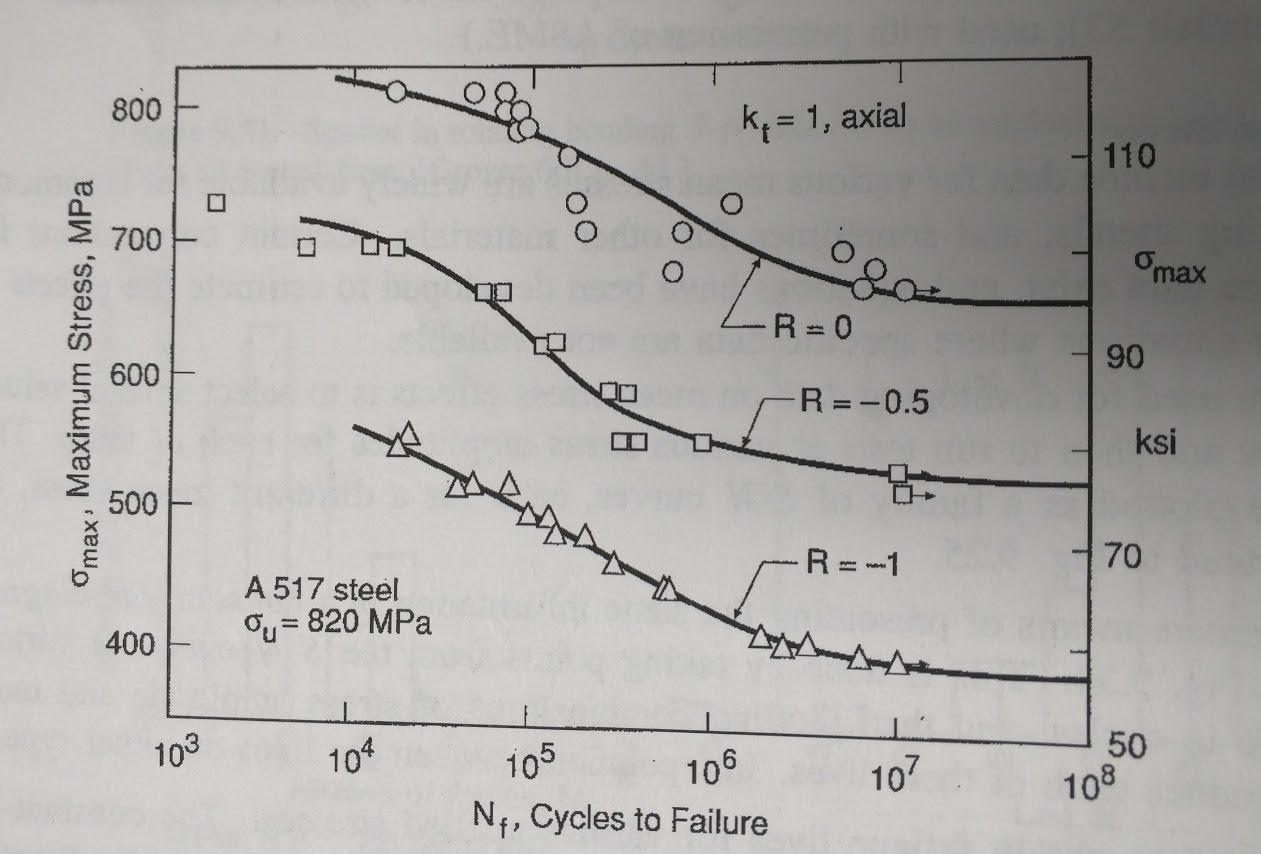
\includegraphics{../images/meanstress.jpg}
\end{frame}

\begin{frame}{constant life diagram}
\protect\hypertarget{constant-life-diagram}{}
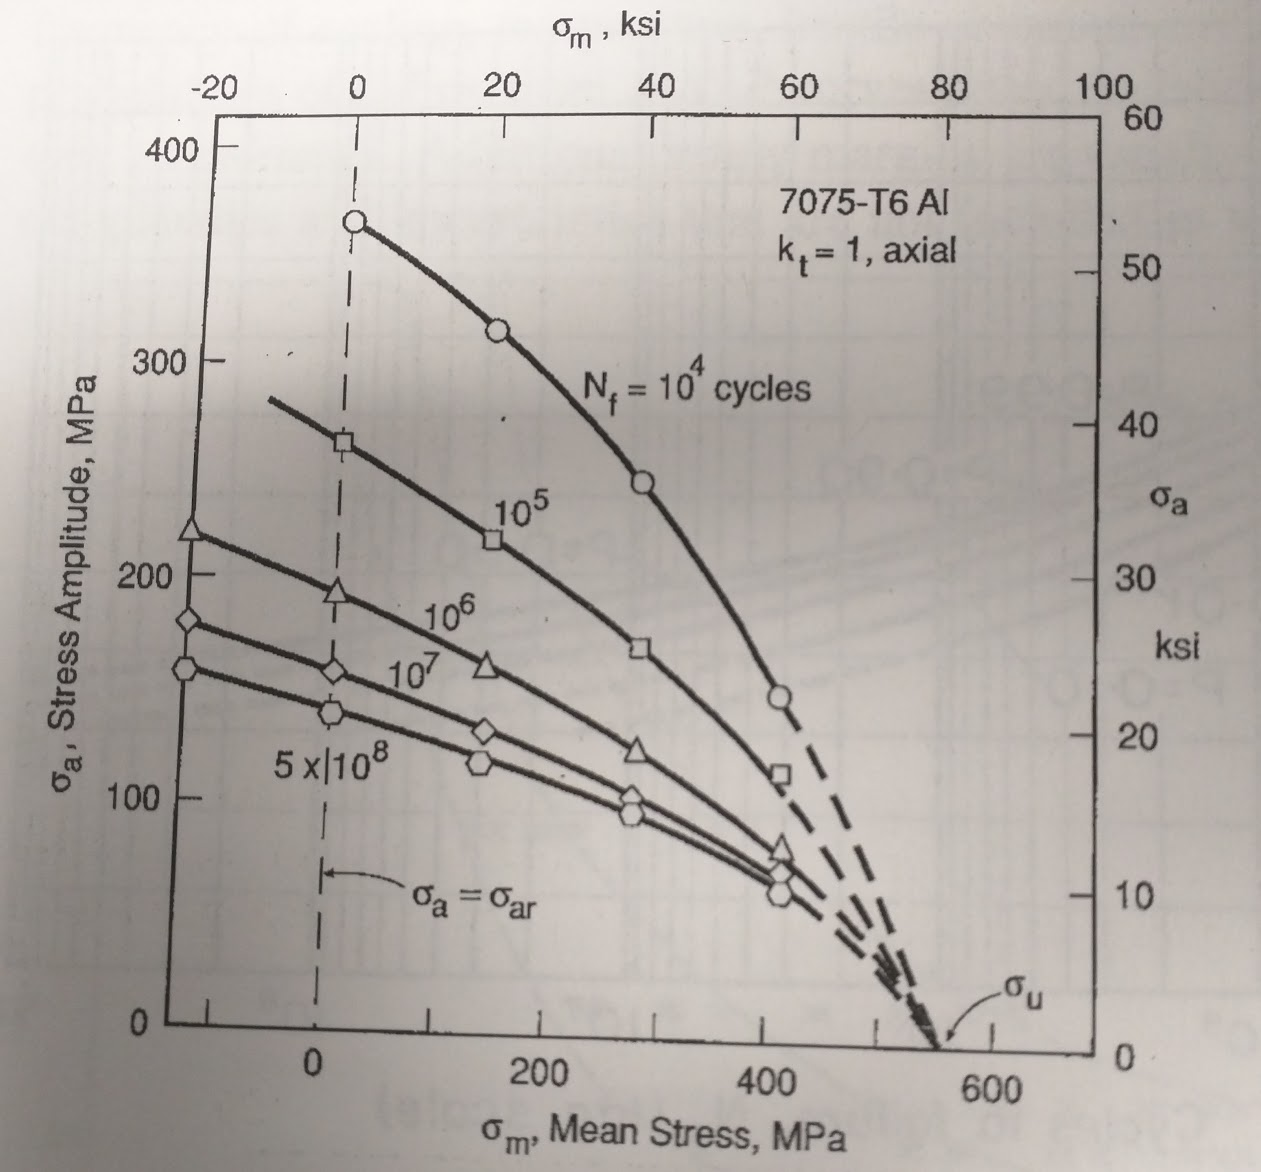
\includegraphics{../images/constant-life.jpg}
\end{frame}

\begin{frame}{normalizing}
\protect\hypertarget{normalizing}{}
\begin{itemize}
\tightlist
\item
  One very useful way to plot this data is to normalize the amplitude by
  the zero-mean amplitude
\item
  We call the zero-mean amplitude \(\sigma_{ar}\)
\item
  Plotting \(\sigma_a/\sigma_{ar}\) vs.~\(\sigma_m\) provides a good way
  to group all the data together on one plot with the potential to fit a
  curve
\end{itemize}
\end{frame}

\begin{frame}{normalized amplitude-mean diagram}
\protect\hypertarget{normalized-amplitude-mean-diagram}{}
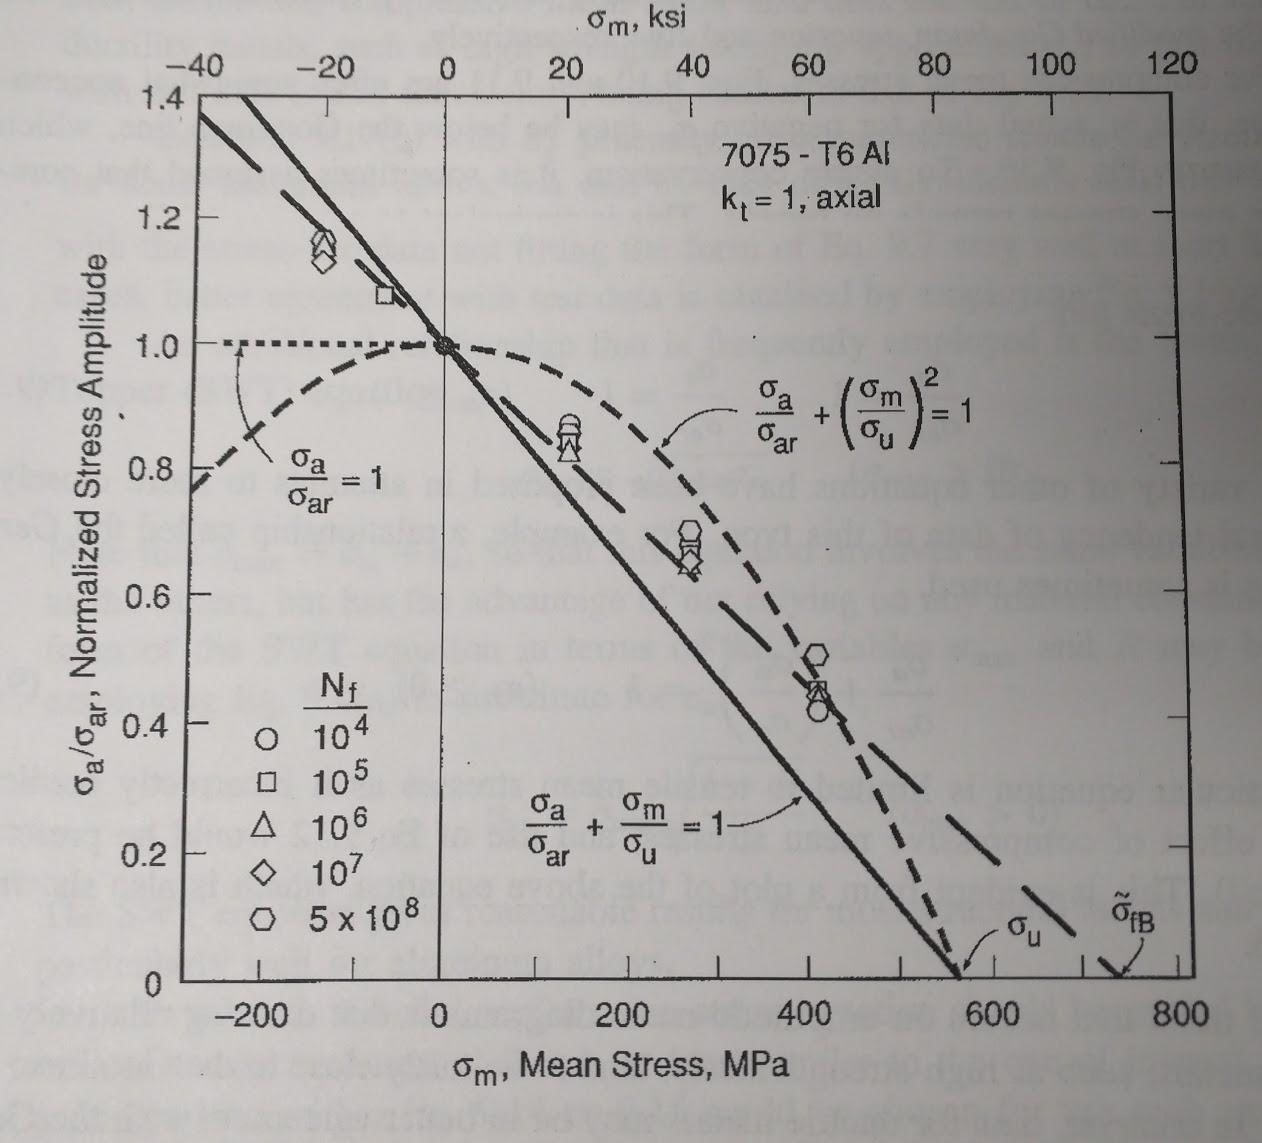
\includegraphics{../images/normalized.jpg}
\end{frame}

\begin{frame}{Goodman line}
\protect\hypertarget{goodman-line}{}
\begin{itemize}
\tightlist
\item
  The first work on this problem was done by Goodman, who proposed the
  line
\end{itemize}

\[\frac{\sigma_a}{\sigma_{ar}} + \frac{\sigma_m}{\sigma_u} = 1\]

\begin{itemize}
\tightlist
\item
  This equation can also be used for fatigue limits, since they are just
  a point on the S-N curves
\end{itemize}

\[\frac{\sigma_e}{\sigma_{er}} + \frac{\sigma_m}{\sigma_u} = 1\]
\end{frame}

\begin{frame}{modifications}
\protect\hypertarget{modifications}{}
\begin{itemize}
\tightlist
\item
  While the Goodman line gives a good approximation to convert non-zero
  mean stress S-N curves, it is somewhat overly conservative at high
  mean stresses
\item
  It is also non-conservative for negative mean stresses
\item
  An alternative fit is known as the Gerber Parabola
\end{itemize}

\[\frac{\sigma_a}{\sigma_{ar}} + \left(\frac{\sigma_m}{\sigma_u}\right)^2 = 1\]

\begin{itemize}
\tightlist
\item
  In general, the Goodman line is a good fit for brittle materials
  (steels) while the Gerber parabola is a better fit for more ductile
  materials
\end{itemize}
\end{frame}

\begin{frame}{modifications}
\protect\hypertarget{modifications-1}{}
\begin{itemize}
\tightlist
\item
  The Goodman line can also be improved by replacing \(\sigma_u\) with
  the corrected true fracture strength \(\tilde{\sigma}_{fB}\) or the
  constant \(\sigma_f^\prime\) from the S-N curve fit
\end{itemize}

\[\frac{\sigma_a}{\sigma_{ar}} + \frac{\sigma_m}{\sigma_f^\prime} = 1\]

\begin{itemize}
\tightlist
\item
  This is known as the Morrow Equation
\item
  For steels, \(\sigma_f^\prime \approx \tilde{\sigma}_{fB}\), but for
  aluminums these values can be significantly different, and better
  agreement is found using \(\tilde{\sigma}_{fB}\).
\end{itemize}
\end{frame}

\begin{frame}{modifications}
\protect\hypertarget{modifications-2}{}
\begin{itemize}
\tightlist
\item
  One more relationship that has shown particularly good results with
  aluminum alloys is the Smith, Watson, and Topper equations (SWT)
\end{itemize}

\[\sigma_{ar} = \sqrt{\sigma_{max}\sigma_a}\]

\begin{itemize}
\tightlist
\item
  In general, it is best to use a form that matches your data
\item
  If data is lacking, the SWT and Morrow equations generally provide the
  best fit
\end{itemize}
\end{frame}

\hypertarget{scatter}{%
\section{scatter}\label{scatter}}

\begin{frame}{fatigue scatter}
\protect\hypertarget{fatigue-scatter}{}
\begin{itemize}
\tightlist
\item
  One of the challenges with fatigue is that there is generally
  considerable scatter in the data
\item
  Quantifying this scatter requires many repetitions, which makes for
  time consuming tests
\item
  In general, the scatter follows a lognormal distribution (or a normal
  distribution in log(\emph{N}\emph{f}))
\end{itemize}
\end{frame}

\begin{frame}{S-N-P Curve}
\protect\hypertarget{s-n-p-curve}{}
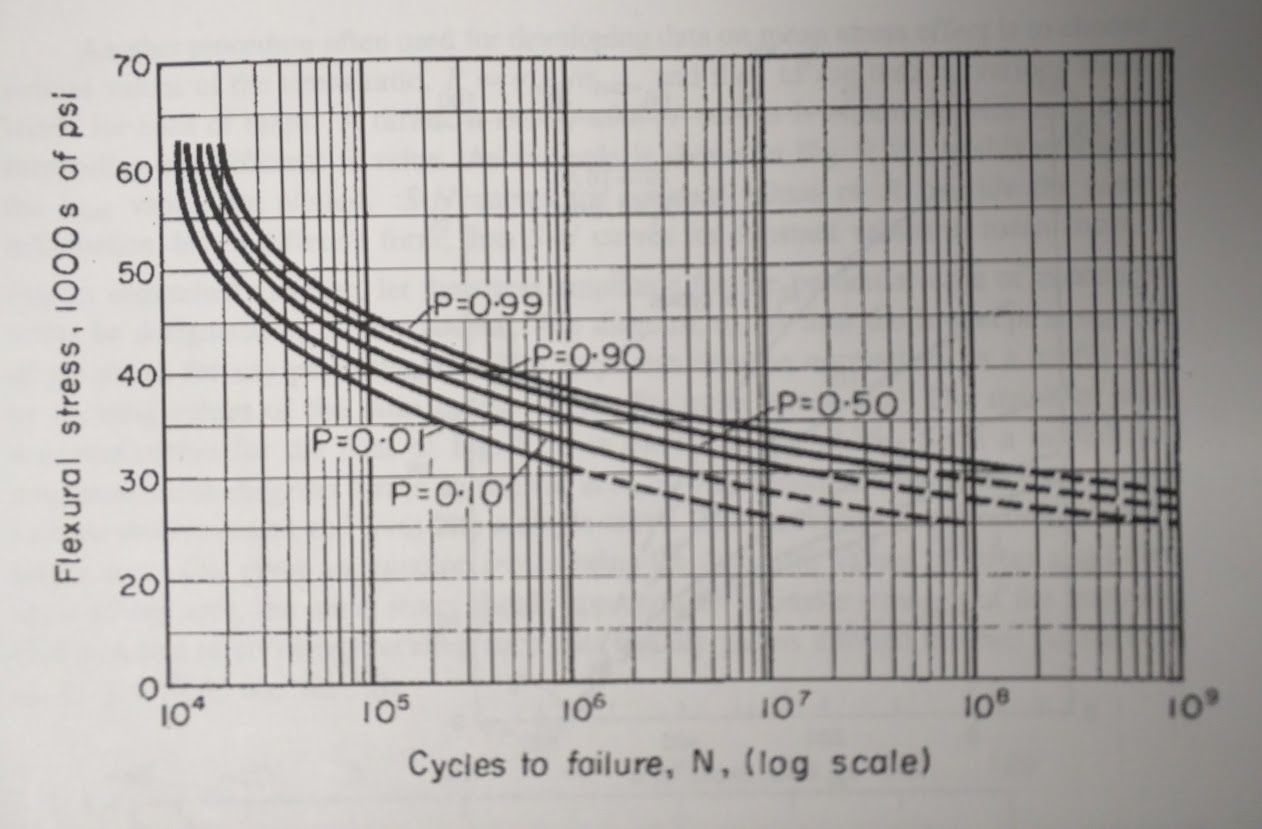
\includegraphics{../images/S-N-P.jpg}
\end{frame}

\hypertarget{general-stress}{%
\section{general stress}\label{general-stress}}

\begin{frame}{general stress}
\protect\hypertarget{general-stress-1}{}
\begin{itemize}
\tightlist
\item
  Often combined loads from different sources introduce stresses which
  are not uni-axial
\item
  For ductile materials, good agreement has been found using an
  effective stress amplitude, similar to the octahedral shear yield
  criterion
\end{itemize}

\[\bar{\sigma}_a = \frac{1}{\sqrt{2}}\sqrt{(\sigma_{xa}-\sigma_{ya})^2 + (\sigma_{ya}-\sigma_{za})^2 + (\sigma_{za}-\sigma_{xa})^2 + 6(\tau_{xy}^2 + \tau_{yz}^2 + \tau_{zx}^2)}\]

\begin{itemize}
\tightlist
\item
  The effective mean stress is given by
\end{itemize}

\[\bar{\sigma}_m = \bar{\sigma}_{xm} + \bar{\sigma}_{ym} + \bar{\sigma}_{zm}\]
\end{frame}

\begin{frame}{effective stress}
\protect\hypertarget{effective-stress}{}
\begin{itemize}
\tightlist
\item
  This effective stress can be used in all other relationships,
  including mean stress relationships
\item
  Note that mean shear stress has no effect on the effective mean stress
\item
  This is surprising, but agrees well with experiments
\item
  When yielding effects do dominate behavior, the strain-based approach
  is more appropriate
\end{itemize}
\end{frame}

\hypertarget{influence-of-notches}{%
\section{influence of notches}\label{influence-of-notches}}

\begin{frame}{notch effects}
\protect\hypertarget{notch-effects}{}
\begin{itemize}
\tightlist
\item
  In this discussion, we use ``notch'' to refer to any geometric feature
  that increases the local stress (such as holes, fillets, grooves,
  etc.)
\item
  We discussed notches and stress concentration factors in terms of
  stress concentration factors
\item
  In our fatigue notation, \(\sigma_{max} = K_t S\)
\item
  This relates local stress to the average, nominal stress
\item
  The stress intensity factor can be used to characterize the
  ``strength'' of a notch
\end{itemize}
\end{frame}

\begin{frame}{notch effects}
\protect\hypertarget{notch-effects-1}{}
\begin{itemize}
\tightlist
\item
  We might expect the fatigue life of a notched specimen to be similar
  to a pristine specimen with
  \(S_{a, pristine} = \sigma_{max, notched}\)
\item
  If we look at actual test data, however, this estimate would be overly
  conservative
\item
  Even when the stress is adjusted for some fatigue notch factor,
  \(k_f\) it is only valid at longer cycles (\(N_f > 10^6\))
\end{itemize}
\end{frame}

\begin{frame}{notch effects}
\protect\hypertarget{notch-effects-2}{}
\[k_f = \frac{\sigma_{ar}}{S_{ar}}\]

\begin{itemize}
\tightlist
\item
  Notches will have different effects, largely depending on their
  radius.
\item
  The maximum possible fatigue notch factor is \(k_f = k_t\)
\end{itemize}
\end{frame}

\begin{frame}{notch effects}
\protect\hypertarget{notch-effects-3}{}
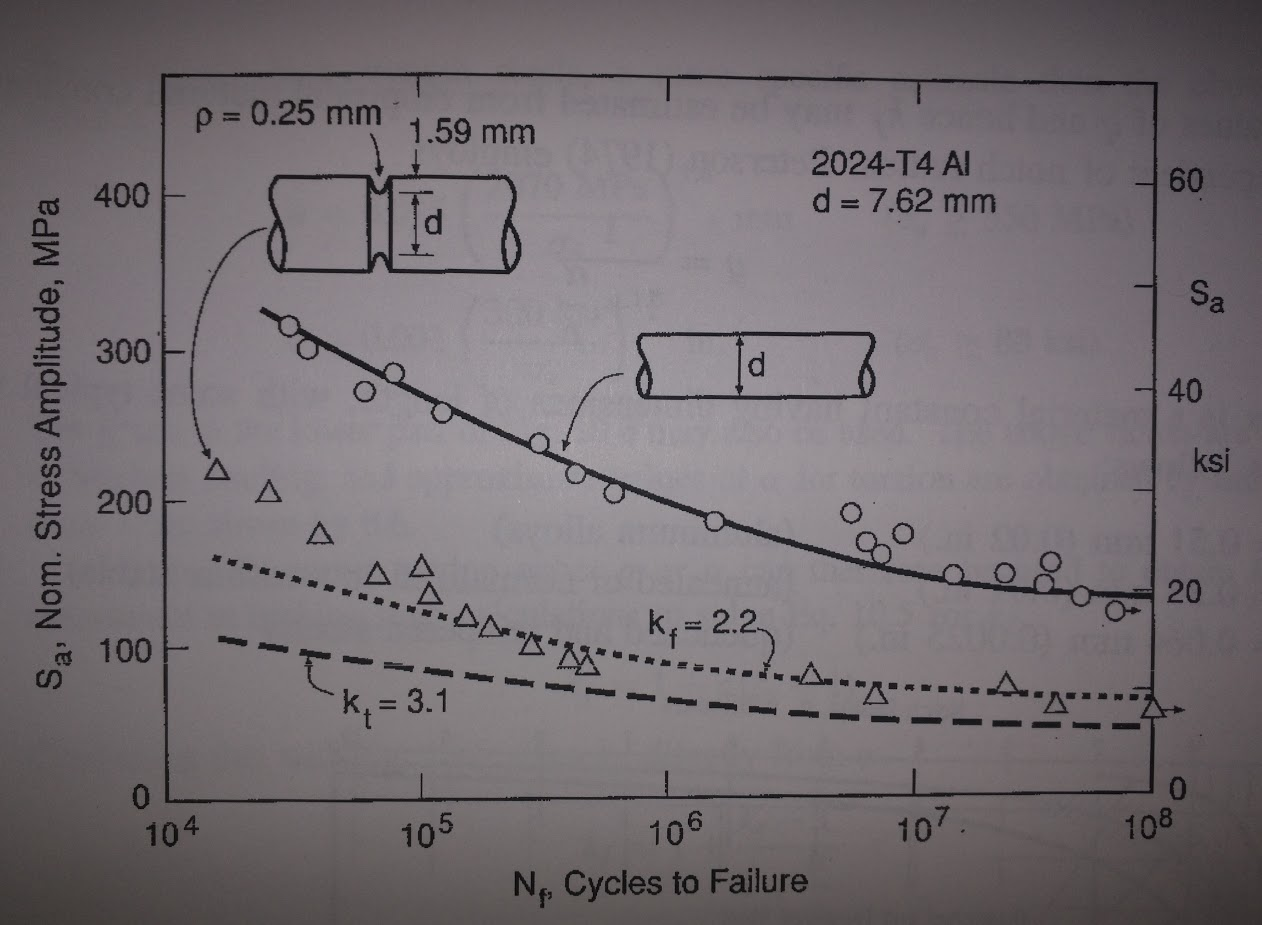
\includegraphics{../images/notch_effect.jpg}
\end{frame}

\begin{frame}{notch sensitivity factor}
\protect\hypertarget{notch-sensitivity-factor}{}
\begin{itemize}
\tightlist
\item
  To avoid generating fatigue data for every possible notch
  configuration, some empirical relationships have been developed
\item
  A useful concept in these methods is the notch sensitivity factor
\end{itemize}

\[q = \frac{k_f - 1}{k_t -1}\]

\begin{itemize}
\tightlist
\item
  When \(k_f = 1\), \(q=0\), in which case the notch has no effect
\item
  When \(k_f = k_t\), \(q=1\), in which case the notch has its maximum
  effect
\end{itemize}
\end{frame}

\begin{frame}{peterson notch sensitivity}
\protect\hypertarget{peterson-notch-sensitivity}{}
\begin{itemize}
\tightlist
\item
  Peterson developed the following relationship
\end{itemize}

\[q = \frac{1}{1+\frac{\alpha}{\rho}}\]

\begin{itemize}
\tightlist
\item
  Where \(\rho\) is the radius of the notch
\item
  \(\alpha\) is a material property
\end{itemize}
\end{frame}

\begin{frame}{peterson notch sensitivity}
\protect\hypertarget{peterson-notch-sensitivity-1}{}
\begin{longtable}[]{@{}ccc@{}}
\toprule
Material & \(\alpha\) (mm) & \(\alpha\) (in) \\ \addlinespace
\midrule
\endhead
Aluminum alloys & 0.51 & 0.02 \\ \addlinespace
Annealed or low-carbon steels & 0.25 & 0.01 \\ \addlinespace
Quenched and tempered steels & 0.064 & 0.0025 \\ \addlinespace
\bottomrule
\end{longtable}
\end{frame}

\begin{frame}{peterson notch sensitivity}
\protect\hypertarget{peterson-notch-sensitivity-2}{}
\begin{itemize}
\tightlist
\item
  For high-strength steels, a more specific \(\alpha\) estimate can be
  found
\end{itemize}

\[\begin{aligned}
  \alpha &= 0.025 \left(\frac{2070 }{\sigma_u}\right)^{1.8} & \text{mm} & \qquad \sigma_u \ge 550 \text{ MPa}\\
  \alpha &= 0.001 \left(\frac{300 }{\sigma_u}\right)^{1.8} & \text{in} & \qquad \sigma_u \ge 80 \text{ ksi}
\end{aligned}\]
\end{frame}

\begin{frame}{peterson notch sensitivity}
\protect\hypertarget{peterson-notch-sensitivity-3}{}
\begin{itemize}
\tightlist
\item
  \(\alpha\) predictions are valid for bending and axial fatigue
\item
  For torsion fatigue, a good estimate can be found
\item
  \(\alpha_{torsion} = 0.6\alpha\)
\end{itemize}
\end{frame}

\begin{frame}{alternative}
\protect\hypertarget{alternative}{}
\begin{itemize}
\tightlist
\item
  An alternative formulation for \emph{q} was developed by Neuber
\end{itemize}

\[q = \frac{1}{1+\sqrt{\frac{\beta}{\rho}}}\]

\begin{itemize}
\tightlist
\item
  Where the material property \(\beta\) for steels is given by
\end{itemize}

\[\begin{aligned}
  \log \beta &= -\frac{\sigma_u - 134}{586} & \text{mm} & \qquad \sigma_u \le 1520 \text{ MPa}\\
  \log \beta &= -\frac{\sigma_u + 100}{85}& \text{in} & \qquad \sigma_u \le 220 \text{ ksi}
\end{aligned}\]
\end{frame}

\begin{frame}{alternative}
\protect\hypertarget{alternative-1}{}
\begin{itemize}
\tightlist
\item
  For aluminum use the chart MPa (ksi) and mm (in.)
\end{itemize}

\begin{longtable}[]{@{}cccc@{}}
\toprule
\endhead
\(S_u\) & 150 (22) & 300 (43) & 600 (87) \\ \addlinespace
\(\beta\) & 2 (0.08) & 0.6 (0.025) & 0.5 (0.015) \\ \addlinespace
\bottomrule
\end{longtable}
\end{frame}

\begin{frame}{notch sensitivity factors}
\protect\hypertarget{notch-sensitivity-factors}{}
\begin{itemize}
\tightlist
\item
  While the above methods are useful, they should be regarded as
  estimates only
\item
  Physical complexities are not fully modeled by these methods
\item
  All of these have been developed for relatively ``mild'' notches
\item
  For sharp notches, best results are found by treating the notch as a
  crack
\end{itemize}
\end{frame}

\begin{frame}{example}
\protect\hypertarget{example}{}
\begin{itemize}
\tightlist
\item
  Find the notch sensitivity factor for the following scenario
\end{itemize}

\[\begin{aligned}
  \rho &= 0.25 \text{ in.}\\
  \sigma_m &= 0 \text{ ksi}\\
  K_t &= 3.0\\
  \sigma_u &= 84 \text{ ksi}
\end{aligned}\]
\end{frame}

\hypertarget{fatigue-review}{%
\section{fatigue review}\label{fatigue-review}}

\begin{frame}{group 1}
\protect\hypertarget{group-1}{}
\begin{itemize}
\tightlist
\item
  A part from AISI 4340 in a typical ``block'' undergoes 100,000 cycles
  with \(\sigma_{min} = 0\) ksi and \(\sigma_{max} = 100\) ksi and an
  additional 10 cycles with \(\sigma_{min} = 50\) ksi and
  \(\sigma_{max} = 200\) ksi
\item
  How many ``blocks'' can this part support before failure?
\end{itemize}
\end{frame}

\begin{frame}{group 2}
\protect\hypertarget{group-2}{}
\begin{itemize}
\tightlist
\item
  Use the S-N-P chart on p.~245 for 7075-T6 Aluminum
\item
  What is the probability of failure for 30 ksi at 106 cycles?
\item
  To ensure that 99\% of parts do not fail, after how many cycles should
  a fully reversed load of 35 ksi be inspected?
\item
  How many cycles could the same part sustain if only 50\% of parts are
  needed?
\end{itemize}
\end{frame}

\begin{frame}{group 3}
\protect\hypertarget{group-3}{}
\begin{itemize}
\tightlist
\item
  The fatigue limit for AISI 4142 steel is 58 ksi for completely
  reversed fatigue loads.
\item
  What is the fatigue limit for fatigue loads with
  \(\sigma_m = 10, 20, 30\) ksi?
\end{itemize}
\end{frame}

\begin{frame}{group 4}
\protect\hypertarget{group-4}{}
\begin{itemize}
\tightlist
\item
  A material made of 2024-T4 Aluminum undergoes the following load cycle

  \begin{itemize}
  \tightlist
  \item
    \(\sigma_{x, min}=10\), \(\sigma_{x, max} = 50\)
  \item
    \(\sigma_{y, min}=-20\), \(\sigma_{x, max} = 20\)
  \item
    \(\tau_{xy, min}=0\), \(\tau_{xy, max} = 30\)
  \end{itemize}
\item
  How many cycles can it support before failure?
\end{itemize}
\end{frame}

\hypertarget{strain-based-fatigue}{%
\section{strain based fatigue}\label{strain-based-fatigue}}

\begin{frame}{strain based fatigue}
\protect\hypertarget{strain-based-fatigue-1}{}
\begin{itemize}
\tightlist
\item
  The strain based fatigue method uses local stresses and strains
  (instead of global, nominal values)
\item
  The strain-based method gives greater detail, and validity at lower
  cycles
\item
  It is still valid for high cycle fatigue (but gives same result as
  stress-based fatigue)
\item
  Does not include crack growth analysis or fracture mechanics
\end{itemize}
\end{frame}

\begin{frame}{strain life curve}
\protect\hypertarget{strain-life-curve}{}
\begin{itemize}
\tightlist
\item
  Similar to the S-N curves in stress-based fatigue analysis, we can
  plot the cyclic strain amplitude vs.~number of cycles to failure
\item
  This is most commonly done using axial test machines (instead of
  rotating bending tests)
\item
  The test is run in strain control (not load control)
\item
  Generally plotted on log-log scale
\end{itemize}
\end{frame}

\begin{frame}{plastic and elastic strain}
\protect\hypertarget{plastic-and-elastic-strain}{}
\begin{itemize}
\tightlist
\item
  We can separate the total strain into elastic and plastic components
\end{itemize}

\textbackslash{[} \epsilon\emph{a = \epsilon}\{ea\} +
\epsilon\_\{pa\}\$`
\end{frame}

\begin{frame}{plastic strain}
\protect\hypertarget{plastic-strain}{}
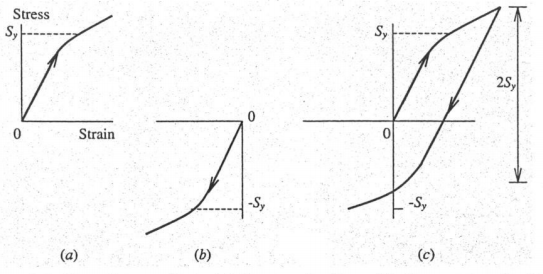
\includegraphics{../images/plastic_strain.PNG}
\end{frame}

\begin{frame}{hysteresis loops}
\protect\hypertarget{hysteresis-loops}{}
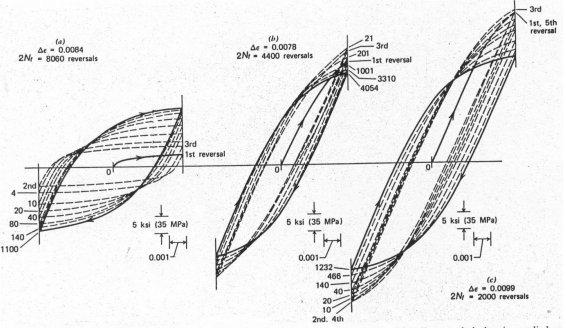
\includegraphics{../images/hysteresis_loops.PNG}
\end{frame}

\begin{frame}{cyclic stress strain curve}
\protect\hypertarget{cyclic-stress-strain-curve}{}
\begin{itemize}
\tightlist
\item
  While strain-life data will generally just report \(\epsilon_a\) and
  \(\epsilon_{pa}\) some will also tabulate a form for the cyclic
  stress-strain curve
\end{itemize}

\[\epsilon_a = \frac{\sigma_a}{E} + \left(\frac{\sigma_a}{H^\prime}\right)^{\frac{1}{n^\prime}}\]
\end{frame}

\begin{frame}{plastic and elastic strain}
\protect\hypertarget{plastic-and-elastic-strain-1}{}
\begin{itemize}
\tightlist
\item
  On strain life curves, the strain is often plotted three times per
  each experiment
\item
  Once for total strain, once for plastic strain, and once for elastic
  strain
\item
  Since plastic strain and elastic strain vary by the number of cycles,
  a hysteresis loop from half the fatigue life is generally used
\item
  This is considered representative of stable behavior
\end{itemize}
\end{frame}

\begin{frame}{experimental data}
\protect\hypertarget{experimental-data}{}
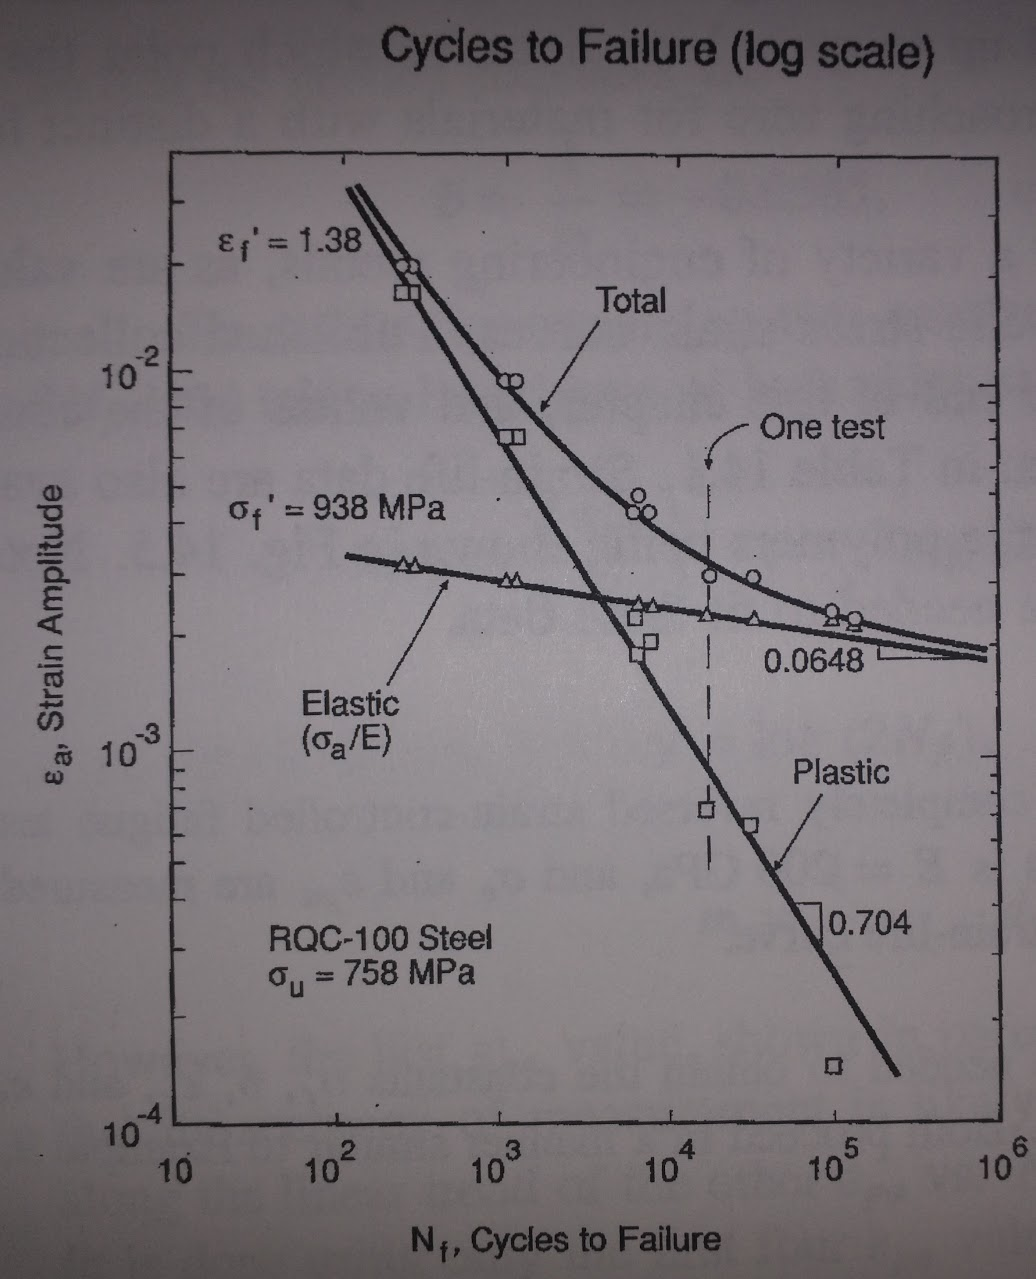
\includegraphics{../images/strain-life.jpg}
\end{frame}

\begin{frame}{trends}
\protect\hypertarget{trends}{}
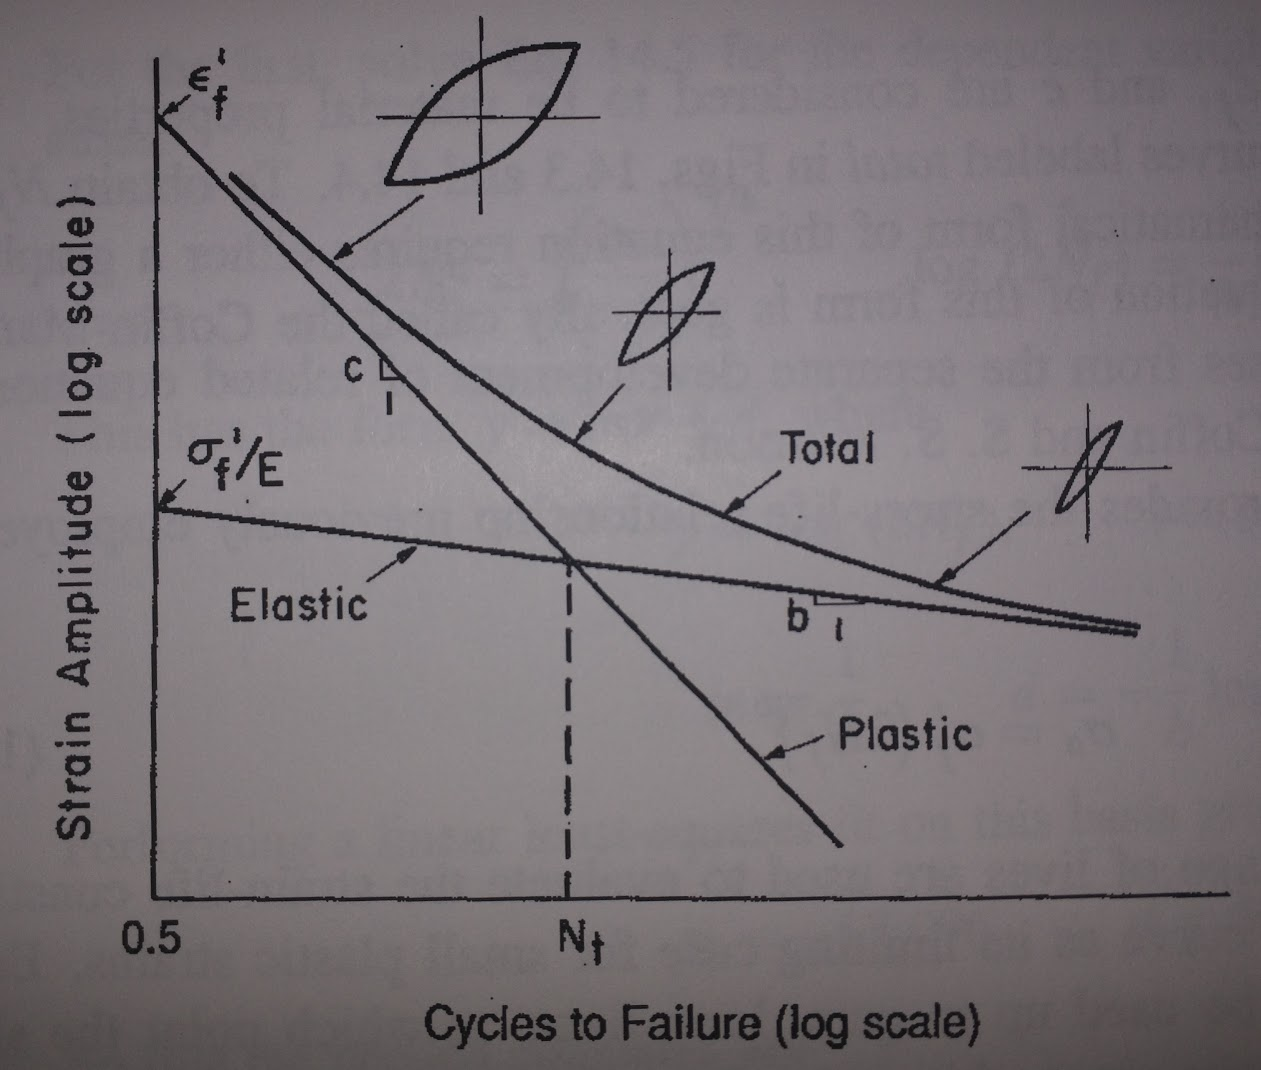
\includegraphics{../images/elastic-plastic.jpg}
\end{frame}

\begin{frame}{lines}
\protect\hypertarget{lines}{}
\begin{itemize}
\tightlist
\item
  We notice that the data for elastic and plastic strains are
  represented by straight lines, in the log-log scale
\item
  If we recall the form used for a straight line in log-log plots for
  S-N curves:
\item
  \(\sigma_a = \sigma_f^\prime (2 N_f)^b\)
\item
  We can convert this to find the elastic component of strain
\end{itemize}

\[\epsilon_{ea} = \frac{\sigma_f^\prime}{E} (2N_f)^b\]
\end{frame}

\begin{frame}{lines}
\protect\hypertarget{lines-1}{}
\begin{itemize}
\tightlist
\item
  We can use the same form with new constants for the plastic component
  of strain
\item
  \(\epsilon_{pa} = \epsilon_f^\prime(2N_F)^c\)
\item
  We can combine the elastic and plastic portions to find the total
  strain-life curve
\end{itemize}

\[\epsilon_a = \frac{\sigma_f^\prime}{E} (2N_f)^b + \epsilon_f^\prime (2 N_f)^c\]
\end{frame}

\begin{frame}{example}
\protect\hypertarget{example-1}{}
\begin{longtable}[]{@{}cccr@{}}
\toprule
\(\epsilon_a\) & \(\sigma_a\) (MPa) & \(\epsilon_{pa}\) &
\(N_f\) \\ \addlinespace
\midrule
\endhead
0.0202 & 631 & 0.01695 & 227 \\ \addlinespace
0.0100 & 574 & 0.00705 & 1030 \\ \addlinespace
0.0045 & 505 & 0.00193 & 6450 \\ \addlinespace
0.0030 & 472 & 0.00064 & 22250 \\ \addlinespace
0.0023 & 455 & (0.00010) & 110000 \\ \addlinespace
\bottomrule
\end{longtable}
\end{frame}

\begin{frame}{transition life}
\protect\hypertarget{transition-life}{}
\begin{itemize}
\tightlist
\item
  With the strain-based fatigue method we are better equipped to discuss
  the difference between high and low-cycle fatigue
\item
  Low-cycle fatigue is dominated by plastic effects, while high-cycle
  fatigue has little plasticity
\item
  We can find the intersection of the plastic strain and elastic strain
  lines
\item
  This point is \(N_t\), the transition fatigue life
\end{itemize}

\[N_t = \frac{1}{2}\left(\frac{\sigma_f^\prime}{\epsilon_f^\prime}\right)^{\frac{1}{c-b}}\]
\end{frame}

\begin{frame}{inconsistencies in constants}
\protect\hypertarget{inconsistencies-in-constants}{}
\begin{itemize}
\tightlist
\item
  If we consider the equation for the cyclic stress train curve
\end{itemize}

\[\epsilon_a = \frac{\sigma_a}{E} + \left(\frac{\sigma_a}{H^\prime}\right)^{\frac{1}{n^\prime}}\]

\begin{itemize}
\tightlist
\item
  We can consider the plastic portion and solve for \(\sigma_a\)
\item
  \(\sigma_a = H^\prime \epsilon_{pa}^n^\prime\)
\end{itemize}
\end{frame}

\begin{frame}{inconsistencies in constants}
\protect\hypertarget{inconsistencies-in-constants-1}{}
\begin{itemize}
\tightlist
\item
  We can eliminate \(2N_f\) from the plastic strain equation
\item
  \(\epsilon_{pa} = \epsilon_f^\prime(2N_f)^c\)
\item
  By solving the stress-life relationship for \(2N_f\)
\item
  \(\sigma_a = \sigma_f^\prime (2NF)^b\)
\item
  and substituting that into the plastic strain
\end{itemize}
\end{frame}

\begin{frame}{inconsistencies in constants}
\protect\hypertarget{inconsistencies-in-constants-2}{}
\begin{itemize}
\tightlist
\item
  We then compare with stress-life equations and find
\end{itemize}

\[\begin{aligned}
 H^\prime &= \frac{\sigma_f^\prime}{(\epsilon_f^\prime)^{b/c}}\\
 n^\prime &= \frac{b}{c}
\end{aligned}\]
\end{frame}

\begin{frame}{inconsistencies in constants}
\protect\hypertarget{inconsistencies-in-constants-3}{}
\begin{itemize}
\tightlist
\item
  However, in practice these constants are fit from different curves
\item
  In some cases there can be large inconsistencies in these values
\item
  One cause for this is data that do not lie on a straight line in the
  log-log domain
\item
  For ductile materials at short lives, the true stresses and strains
  may differ significantly from engineering stress and strain
\end{itemize}
\end{frame}

\hypertarget{variable-amplitude-strains}{%
\section{variable amplitude strains}\label{variable-amplitude-strains}}

\begin{frame}{variable amplitude strains}
\protect\hypertarget{variable-amplitude-strains-1}{}
\begin{itemize}
\tightlist
\item
  As with stresses, we can apply variable amplitude strains
\item
  However, when the change is made will affect whether there is a
  tensile or compressive mean stress
\end{itemize}
\end{frame}

\begin{frame}{compressive mean}
\protect\hypertarget{compressive-mean}{}
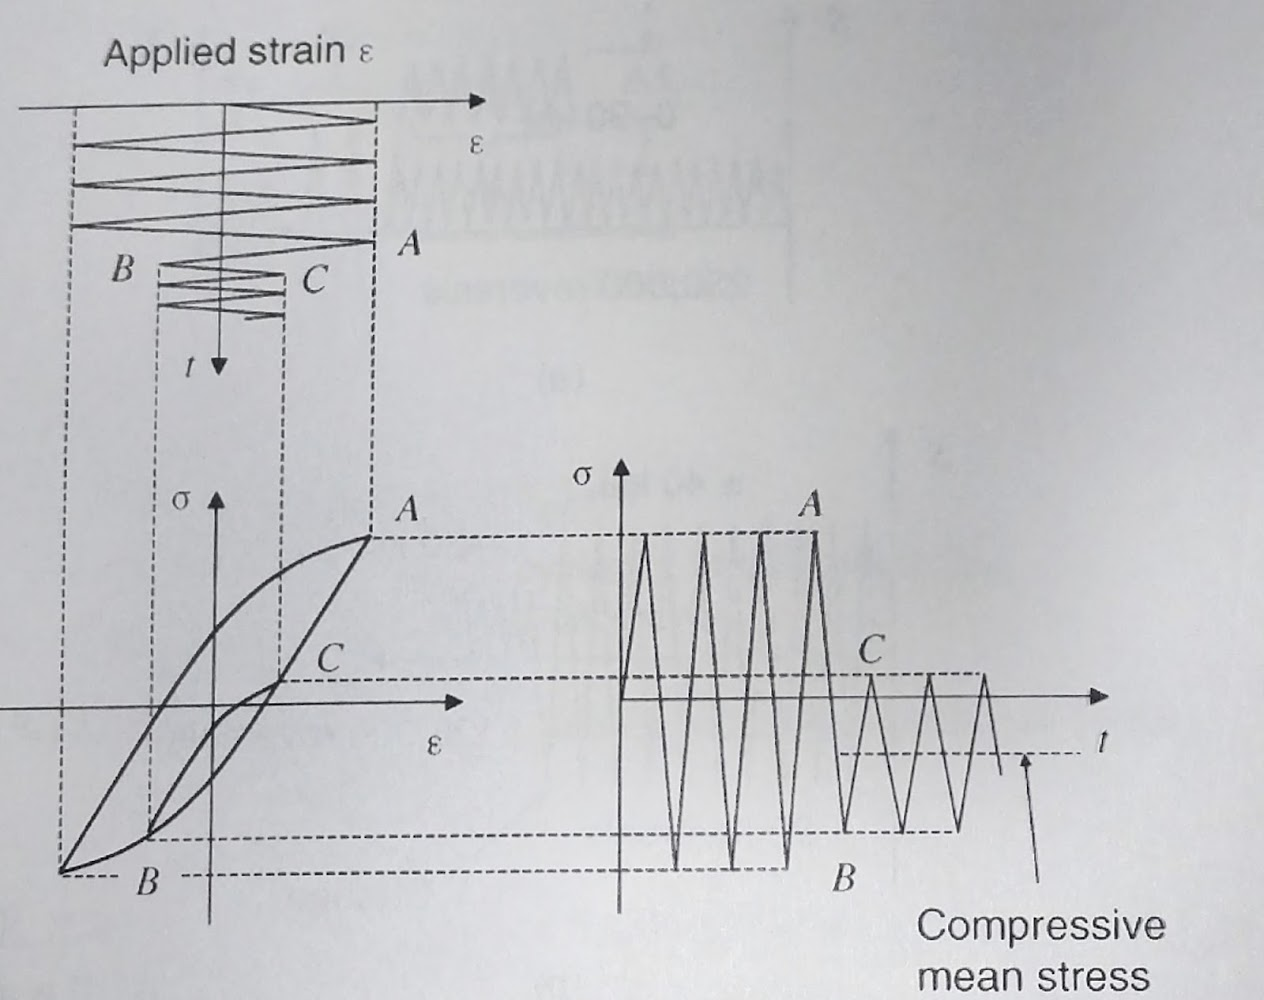
\includegraphics{../images/compressive_mean.jpg}
\end{frame}

\begin{frame}{tensile mean}
\protect\hypertarget{tensile-mean}{}
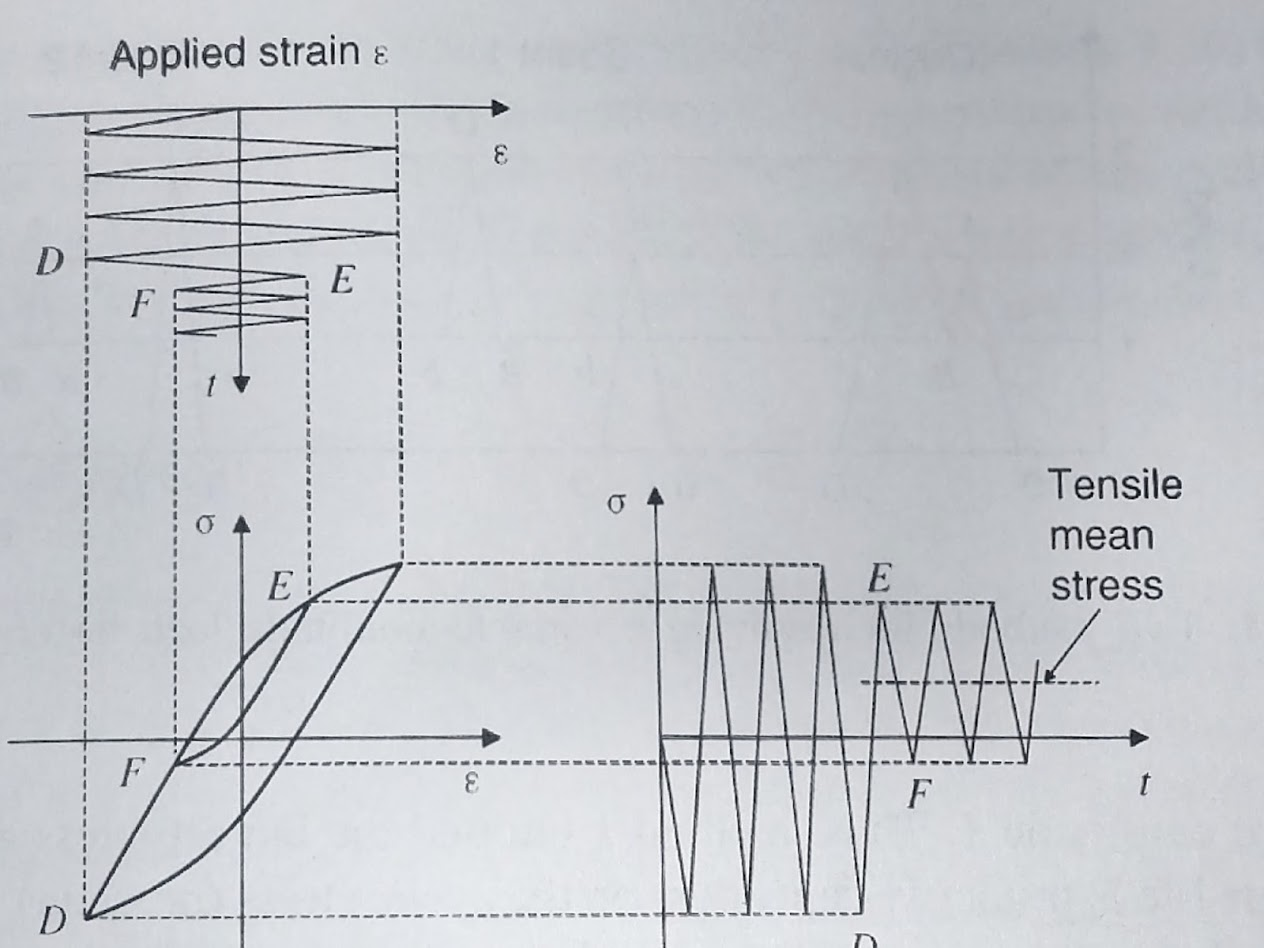
\includegraphics{../images/tensile_mean.jpg}
\end{frame}

\begin{frame}{cycle counting}
\protect\hypertarget{cycle-counting}{}
\begin{itemize}
\tightlist
\item
  In all fatigue methods (stress, strain, and crack propagation) the way
  we count load cycles can have an effect on our results
\item
  To avoid being non-conservative, we need to always count the largest
  amplitudes first
\item
  We will discuss some specific cycle-counting algorithms during crack
  propagation
\end{itemize}
\end{frame}

\begin{frame}{cycle counting}
\protect\hypertarget{cycle-counting-1}{}
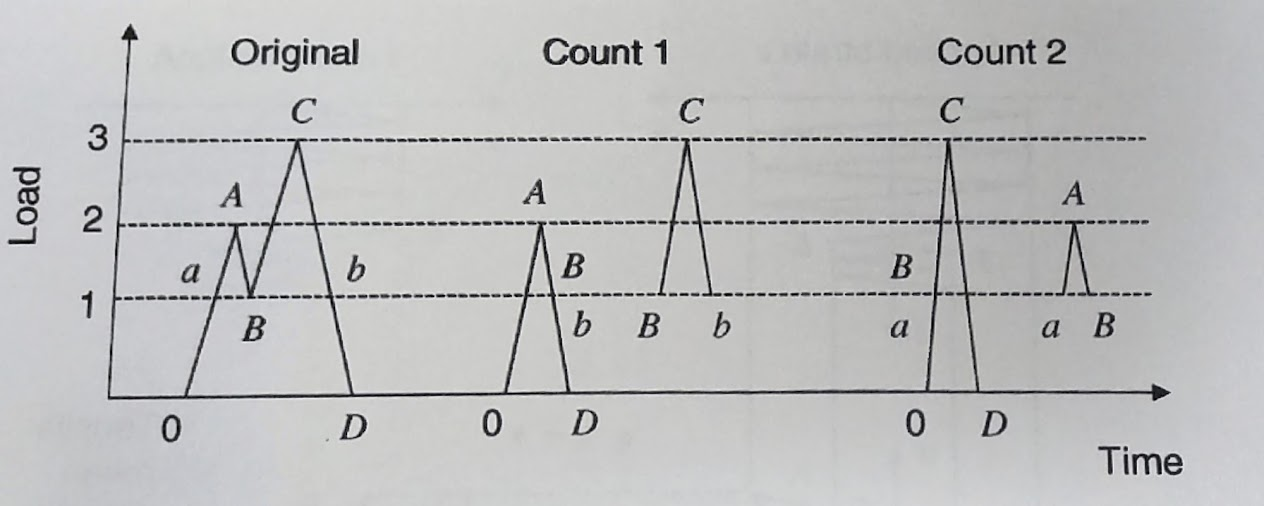
\includegraphics{../images/cycle_counting.jpg}
\end{frame}

\hypertarget{general-trends}{%
\section{general trends}\label{general-trends}}

\begin{frame}{true fracture strength}
\protect\hypertarget{true-fracture-strength}{}
\begin{itemize}
\tightlist
\item
  We can consider a tensile test as a fatigue test with \(N_f = 0.5\)
\item
  We would then expect the true fracture strength
  \(\tilde{\sigma}_f \approx \sigma_f^\prime\)
\item
  And similarly for strain
  \(\tilde{\epsilon}_f \approx \epsilon_f^\prime\)
\end{itemize}
\end{frame}

\begin{frame}{ductile materials}
\protect\hypertarget{ductile-materials}{}
\begin{itemize}
\tightlist
\item
  Since ductile materials experience large strains before failure, we
  expect relatively large \emph{ϵ}\emph{f}′ and relatively small
  \(\sigma_f^\prime\)
\item
  This will cause a less steep slope in the plastic strain line
\item
  In turn this intersects with the elastic strain line much later,
  resulting a longer transition life for ductile materials
\end{itemize}
\end{frame}

\begin{frame}[fragile]{brittle materials}
\protect\hypertarget{brittle-materials}{}
\begin{itemize}
\tightlist
\item
  Brittle materials exhibit the opposite effect, with relatively low
  \(\epsilon_f^\prime\) and relatively high
  \texttt{\textbackslash{}sigma\_f\^{}\textbackslash{}prime}
\item
  This results in a steeper plastic strain line
\item
  And shorter transition life
\end{itemize}
\end{frame}

\begin{frame}{tough materials}
\protect\hypertarget{tough-materials}{}
\begin{itemize}
\tightlist
\item
  Tough materials have intermediate values for both
  \(\epsilon_f^\prime\) and \(\sigma_f^\prime\)
\item
  This gives a transition life somewhere between brittle and ductile
  materials
\item
  It is also noteworthy that strain-life for many metals pass through
  the point \(\epsilon_a = 0.01\) and \(N_f = 1000\) cycles
\item
  Steels also follow a trend with Brinell Hardness, the higher they are
  on the HB scale, the lower their transition life
\end{itemize}
\end{frame}

\begin{frame}{typical property ranges}
\protect\hypertarget{typical-property-ranges}{}
\begin{itemize}
\tightlist
\item
  Most common engineering materials have \(-0.8 < c < -0.5\), most
  values being very close to \emph{c} = −0.6
\item
  The elastic strain slope generally has \emph{b} = −0.085
\item
  A ``steep'' elastic slope is around \emph{b} = −0.12, common in soft
  metals
\item
  While ``shallow'' slopes are around \emph{b} = −0.05, common for
  hardened metals
\end{itemize}
\end{frame}

\end{document}
